\documentclass[12pt]{article}

\usepackage{fullpage}
\usepackage{multicol,multirow}
\usepackage{tabularx}
\usepackage{listings}
\usepackage{pgfplots}
\usepackage[utf8]{inputenc}
\usepackage[russian]{babel}
\usepackage[T2A]{fontenc}
\usepackage{pgfplots}
\usepackage{tikz}


\begin{document}

% \newpage
% \begin{center}
% {\bfseries ФЕДЕРАЛЬНОЕ ГОСУДАРСТВЕННОЕ БЮДЖЕТНОЕ ОБРАЗОВАТЕЛЬНОЕ\\
% УЧРЕЖДЕНИЕ ВЫСШЕГО ОБРАЗОВАНИЯ\\
% «МОСКОВСКИЙ АВИАЦИОННЫЙ ИНСТИТУТ\\
% (НАЦИОНАЛЬНЫЙ ИССЛЕДОВАТЕЛЬСКИЙ УНИВЕРСИТЕТ)»}
% \vspace{1cm}

% Журнал лабораторных работ
% \vspace{6em}

% \vspace{\fill}

% \begin{center}
% Москва 2024
% \newpage
% \end{center}

\section*{Лабораторная работа №4\, по курсу компьютерной графики}

\textbf{Тема:} Освещение и работа с шейдерами\\
\\
\textbf{Задача:} Научиться работать с освещением в 3D-пространстве, используя различные типы источников света, и освоить основы написания шейдеров. 
Нужно реализовать освещение объектов в сцене с использованием простейших моделей освещения и настроить эффект при помощи вершинных и фрагментных шейдеров.\\
\textbf{Вариант:} 2. \\
Постройте сферу в 3D-пространстве.\\
Реализуйте точечный источник света (Point Light), используя модель Фонга для освещения.\\
Включите зеракльные блики (Specular Highlights) для более реалистичнго отражения света на поверхности объекта.\\
Дополнительно: Добавьте управление положением источника света с помощью клавиатуры.\\

\subsection*{1 Решение}
Для выполнения лабораторной работы 4 я использовал OpenGL для реализации освещения в 3D-пространстве. 
Реализовал точечный источник света и написал шейдер с использованием модели Фонга для расчёта освещенности объектов. 
Добавил зеркальные блики для более реалистичного отображения. 
Также обеспечил управление положением источника света с помощью клавиш.

\begin{figure}[h]

\centering
        
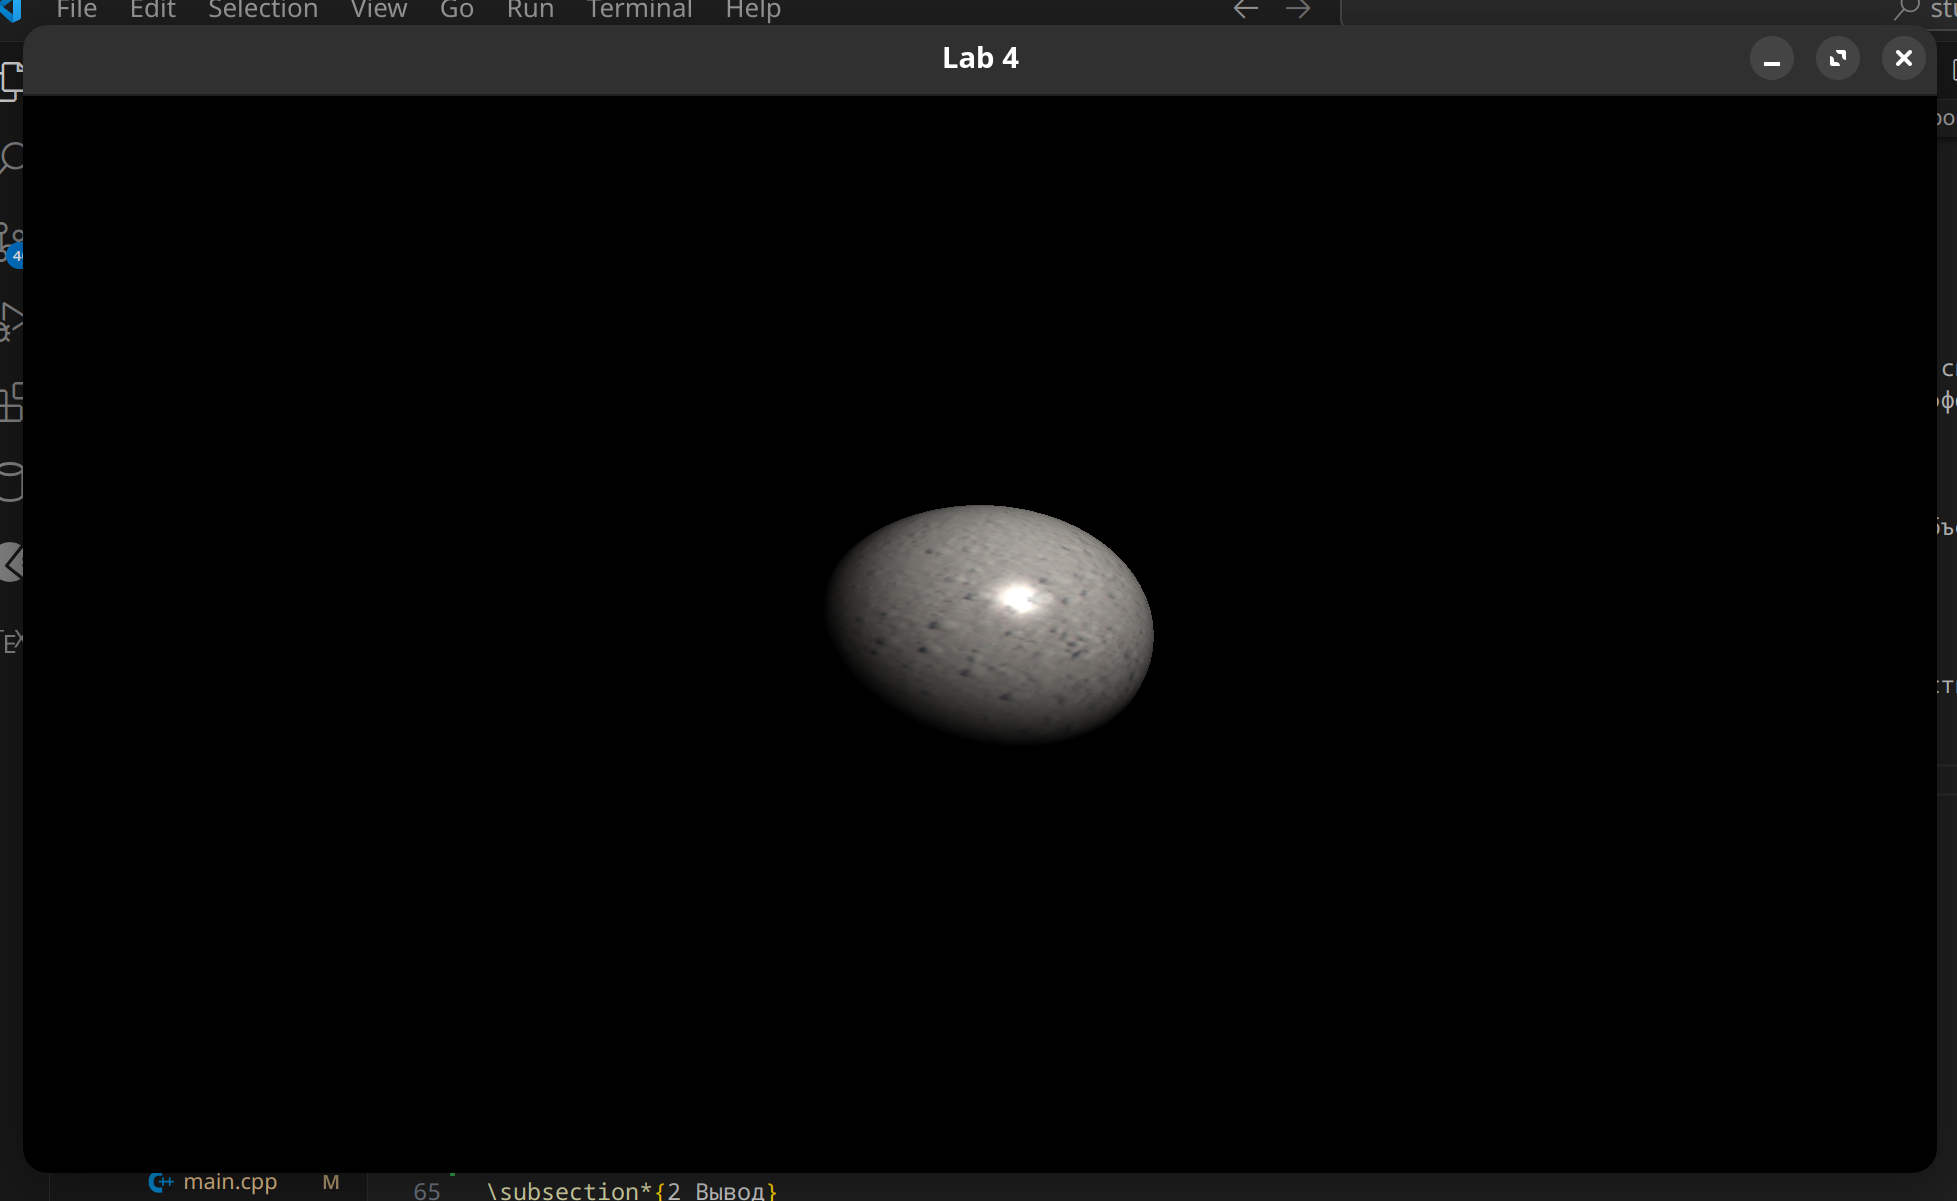
\includegraphics[width=0.8\linewidth]{image.png}
        
\caption{Пример работы программы}
        
\label{fig:mpr}
        
\end{figure}

\subsection*{2 Вывод}
В ходе лабораторной работы 4 была реализована система освещения в 3D-пространстве с использованием модели Фонга, что позволило добавить реалистичные эффекты освещенности и зеркальных бликов. 
Также была реализована возможность управления источником света, что улучшило взаимодействие с 3D-сценой. 
Работа позволила углубить знания о 3D-графике и освещении объектов в OpenGL.
\end{document}
